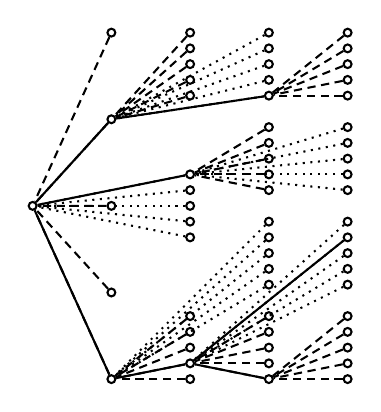
\begin{tikzpicture}
[font=\footnotesize, draw=black, line width=0.75pt,
fragment/.style={circle, draw, inner sep=0pt, minimum size=1mm}]

\node[fragment,minimum size=1mm] (x0y0) at (0, 2) {};

\foreach \y in {0, ..., 4} {
    \node[fragment] (x1y\y) at (1, -0.2+1.1*\y) {}
        edge[densely dashed] (x0y0);
}
\draw (x0y0) -- (x1y0);
\draw (x0y0) -- (x1y3);

\foreach \y in {0, ..., 4} {
    \node[fragment] (x2ys\y) at (2, 1.6+0.2*\y) {}
        edge[dotted] (x0y0);
}
\draw (x0y0) -- (x2ys4);
\foreach \y in {0, ..., 4} {
    \node[fragment] (x2y0\y) at (2, -0.2+0.2*\y) {}
            edge[densely dashed] (x1y0);
}
\draw (x1y0) -- (x2y01);
\foreach \y in {0, ..., 4} {
    \node[fragment] (x2y3\y) at (2, 3.4+0.2*\y) {}
            edge[densely dashed] (x1y3);
}


\foreach \y in {0, ..., 4} {
        \node[fragment] (x3y01\y) at (3, -0.2+0.2*\y) {}
            edge[densely dashed] (x2y01);
}
\draw (x2y01) -- (x3y010);
\foreach \y in {0, ..., 4} {
        \node[fragment] (x3y0s\y) at (3, 1+0.2*\y) {}
            edge[dotted] (x1y0);
}
\foreach \y in {0, ..., 4} {
        \node[fragment] (x3ys4\y) at (3, 2.2+.2*\y) {}
            edge[densely dashed] (x2ys4);
}
\foreach \y in {0, ..., 4} {
        \node[fragment] (x3y3s\y) at (3, 3.4+0.2*\y) {}
            edge[dotted] (x1y3);
}
\draw (x1y3) -- (x3y3s0);

\foreach \y in {0, ..., 4} {
        \node[fragment] (x4y010\y) at (4, -0.2+0.2*\y) {}
            edge[densely dashed] (x3y010);
}
\foreach \y in {0, ..., 4} {
        \node[fragment] (x4y01s\y) at (4, 1+0.2*\y) {}
            edge[dotted] (x2y01);
}
\draw (x2y01) -- (x4y01s3);
\foreach \y in {0, ..., 4} {
        \node[fragment] (x4ys4s\y) at (4, 2.2+.2*\y) {}
            edge[dotted] (x2ys4);
}
\foreach \y in {0, ..., 4} {
        \node[fragment] (x4y3s2\y) at (4, 3.4+0.2*\y) {}
            edge[densely dashed] (x3y3s0);
}

\end{tikzpicture}
